% !TEX root = OptimalOffline.tex

\begin{figure}
\label{lemma4}
\centering
  \centerline{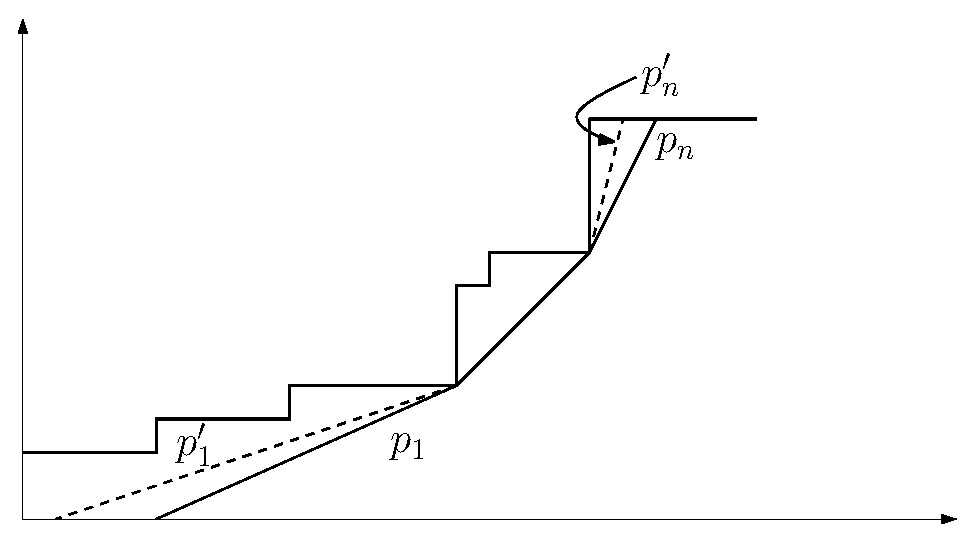
\includegraphics[width=8cm,height=50mm]{Lemma4.eps}}
\caption{Illustration of the proof of lemma \ref{transmission_duration}. The dotted line represents the policy where the first power of transmission is slightly reduced, to make the transmissino finish earlier}
\end{figure}

\begin{lemma}
If the receiver has enough energy to stay on for $T$ time, then either the transmitter will transmit for the entire duration $T$ or the transmitter will begin transmission at time $t=0$.
\label{transmission_duration}
\end{lemma}
\begin{proof}
We will prove this by contradiction. Suppose the optimal transmission policy $\{\textbf{p},\textbf{s},N\}$ does not begin transmitting at time $t=0$ and transmits for a duration $s_{N+1}-s_1 < T$.

If we reduce $p_1$ slightly to $p_1-\delta p_1$, we will have transmitted more bits by time $s_N$. Therefore at the end we can transmit with a power $p'_N > p_N$ and complete our transmission at an earlier time.

Thus we can keep lowering our first transmission power until we either exhaust our transmission duration $T$ or we hit the origin.
\end{proof}

Concluding the results of all Lemmas our optimal policy $\{\textbf{p},\textbf{s},N\}$ must have change transmission powers at energy arrival epochs only i.e. $\forall i,\ s_i=t_j$ for some $j$. At these epochs we exhaust the total energy available with us i.e. $U(s_i^-)=\ETx(s_i^-)$. The transmission powers are also non decreasing with time and we exhaust the total 'receiver time' time given to us, if we do not start transmitting from origin.

Now that we have gained some knowledge of the structure our algorithm has to follow, we consider an example to approach Problem 1. 

Suppose we are given that the receiver can be \textit{on} for a maximum duration of $T$. Our goal is to find a transmission policy so that we can minimize the time at which the transmission is completed. To do this, we shall first find a feasible solution i.e. one which satisfies all constraints (\ref{pb1_constraint_bits})-(\ref{pb1_constraint_time}) and keep improving upon it, until we have a solution that follows all our Lemma 1-4 and hits the boundary on some or all of the constraints (\ref{pb1_constraint_bits})-(\ref{pb1_constraint_time}). 

We need an initial feasible solution to begin with. For this, we find the minimum energy required by the transmitter so that the transmission can be completed in duration $T$ with a constant power. That is, the first $n$ such that
\begin{equation}
T g\left(\frac{\ETx(t_n)}{T}\right)\geq B_0.
\end{equation}
Let $\widetilde{T}$ be the time duration such that
\begin{equation}
\widetilde{T}g\left(\frac{\ETx(t_n)}{\widetilde{T}}\right)=B_0.
\end{equation}
Let $\tilde{p}=\frac{\ETx(t_n)}{\widetilde{T}}$. We try to transmit with this power starting at t=0. If it does not violate the energy constraint (\ref{pb1_constraint_energy}), we are done with the optimal solution and our transmission is completed in $\widetilde{T}$ time.

If not, we start the transmission as early as possible, such that the transmission is feasible with respect to (\ref{pb1_constraint_energy}). This transmission policy, will encounter atleast one epoch where total energy consumed till that epoch is equal to the total energy harvested upto it. Let time $Q$ be the first point where this happens. This is shown in Figure \ref{straight}. Till now we have not argued why we chose such a policy to start with. In fact the next Lemma shows that this starting solution is a 'good' estimate as both the optimal policy and the above policy run out of all their energy at epoch $Q$.

\begin{figure}
\label{straight}
\centering
  \centerline{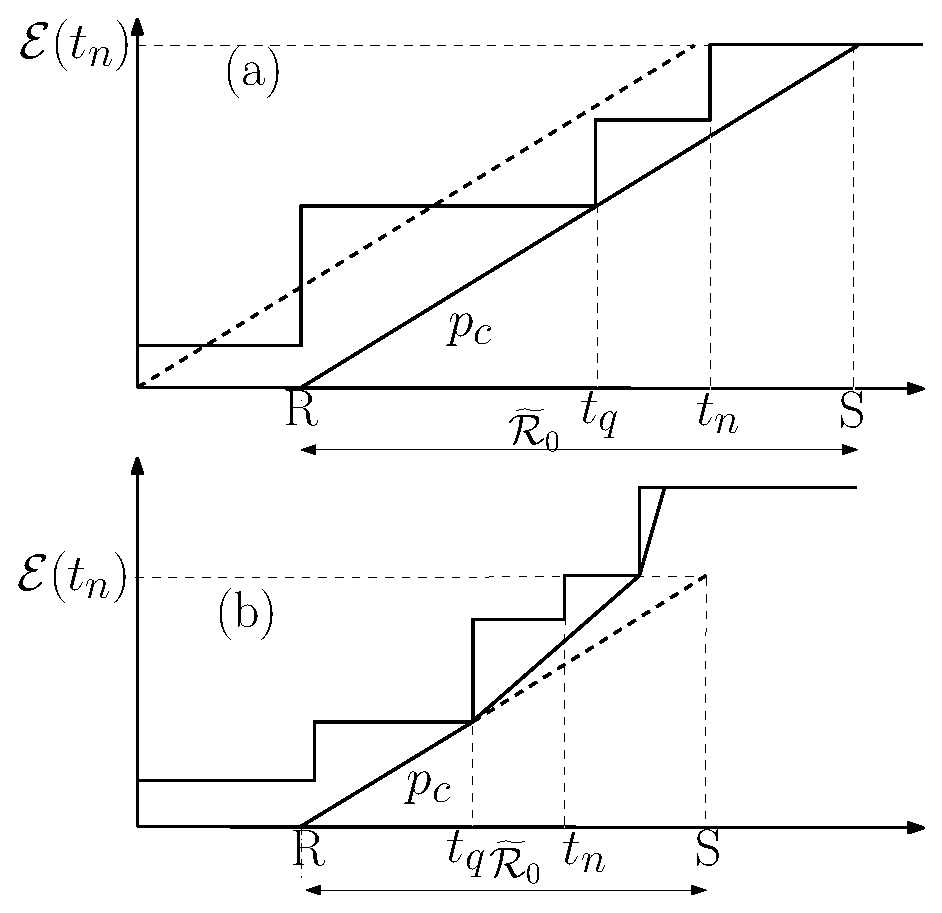
\includegraphics[width=8cm,height=4cm]{straight.eps}}
\caption{Figure showing point Q.}
\end{figure}

\begin{lemma}
In every optimal solution, at energy arrival epoch $Q$, $U(Q^-)=\ETx(Q^-)$.
\label{lemma_Q}
\end{lemma}
\begin{proof}
We shall prove this by contradiction. Let the start and end times of the constant power transmission policy described above be $R$ and $S$ receptively. We make the following claims:

\textbf{Claim 1:} Every optimal transmission policy begins transmission at or before time $R$

Since, $S-T=\widetilde{T}\le T$ (by Lemma \ref{transmission_duration}) if a transmission policy has to finish before $S$, it has to start before time $\max(S-T,0) \le \max(R,0)$. 

%Since we are transmitting all the bits at the maximum possible power, no policy that starts after $R$ can finish before $S$. Therefore, any policy that starts after $R$ cannot be optimal.

\textbf{Claim 2:} Every optimal transmission policy ends transmission at or before time $S$.
This follows immediately from the fact that the policy is optimal.

Let $Q$ equal to time $t_i$ for some $i\in\mathbb{N}$. Suppose we have an optimal transmission policy that does not exhaust all its energy at time $Q$ i.e. $U(t_j)<\ETx(t_i^-)$. By Lemma \ref{lemma_energy_consumed} it does not change its transmission power at $t_i$. Let the transmission power of optimal policy be $p$ at $t_i$. This does not change till an epoch, say $t_j$. Now, $t_j<S$ by \textit{Claim 2}. Further the constant power policy exhausts all its energy by $Q$. So,
\begin{align}
&\tilde{p}(t_i-R)=\ETx(t_i^-)\label{eqlemmaQ1}.
\end{align}
But, by constraint (\ref{pb1_constraint_energy})
\begin{align}
&\tilde{p}(t_i-R)+\tilde{p}(t_j-t_i)\le \ETx(t_j^-),
\\
&\implies \tilde{p}(t_j-t_i)\stackrel{(\ref{eqlemmaQ1})}{\le} \ETx(t_j^-)-\ETx(t_i^-),\\
&\implies \tilde{p}(t_j-t_i)< \ETx(t_j^-)-U(t_i)=p(t_j-t_i),\\
&\implies \tilde{p}<p .\label{eqlemmaQ2}
\end{align}
If the optimal policy does have a power higher than $\tilde{p}$ at $t_i$, then it must have the same power of transmission either from some epoch, say $t_k$, or from the beginning of transmission. If $t_k>R$, we can show that the constant power policy is infeasible with respect to constraint (\ref{pb1_constraint_energy}) at $t_k$. If $t_k<R$ it becomes infeasible at time $R$. If the optimal policy starts transmission with power $p$, it has to begin transmission after time $R$ which follows from equation (\ref{eqlemmaQ2}). This violates \textit{Claim 1}. Therefore every optimal transmission policy must use all energy till epoch $Q$.
\end{proof}

Now that we have a starting feasible solution, we shall proceed to improve upon this policy as follows. Let $t_{lt}$ and $t_{rt}$ be the first and last energy arrival epochs where the power of transmission changes. 
As it is evident, initially both $t_{lt}$ and $t_{rt}$ are set to point $Q$. Now, will iteratively try to omporove on the transmission curve to the left and the right of point $Q$ respectively. 
Keeping in mind Lemma \ref{transmission_duration}, we solve 
\begin{equation}
\label{xandy}
xg\left(\frac{\ETx(t_{lt})}{x}\right) + (T-x)g\left(\frac{\ETx(n)-\ETx(t_{rt})}{T-x}\right) = B_0
\end{equation}
Notice that $t_{lt} - x$ and $t_{rt} + T-x$ will give us the start and end points of this iteration. Now, we transmit at power $p_{lt} = \frac{\ETx(t_{lt})}{x}$ prior to $t_{lt}$ and $p_{rt} = \frac{\ETx(n) - \ETx(t_{rt})}{T-x}$ after $t_{rt}$. 
If this policy is feasible, then we check for the following. First, we make sure that at the end point, all the available energy is used up, because of it isn't, we can transmit at a higher power and finish earlier. 
If all the energy is not used up, we repeat our iteration, setting $n$ to $k$, where $t_k$ is the last energy arrival epoch before our end point, $t_{rt} + T-x$  \\
If all the energy is used up, then we set $t_{rt}$ to the end point. 
Also, we make sure that our start point, is not before the origin. If the start point is negative, we set it to origin. Now if our start point happend to hit origin at any point in the algorithm, then our problem can be 
solved using the algorithm described by Yang et al in \cite{Yang}. So, should our start point hit origin, we simply use their algorithm for the allocations beyond $t_{rt}$.

If the policy is unfeasible on the right, we select the corner point $t_i$ with the minimum slope from $t_{rt}$ and transmit with power $\frac{\ETx(t_i) - \ETx(t_{rt})}{t_i-t_{rt}}$ between the two points and set $t'_{rt} = t_{rt}$ and $t_{rt} = t_i$ and repeat the process.\\
If the policy is unfeasible on the left, we follow a similar process, be selecting the corner point $t_j$ with the \textit{maximum} slope from point $t_{rt}$.\\
At the end of every iteration we reset our $T$ to $ T - (t_{rt} - t'_{rt}) - (t'_{lt} - t_{lt})$ and we subtract the number of bits transferred between $t_{lt}$ and $t_{rt}$ from $B$

\begin{figure}
\label{theorem1}
\centering
  \centerline{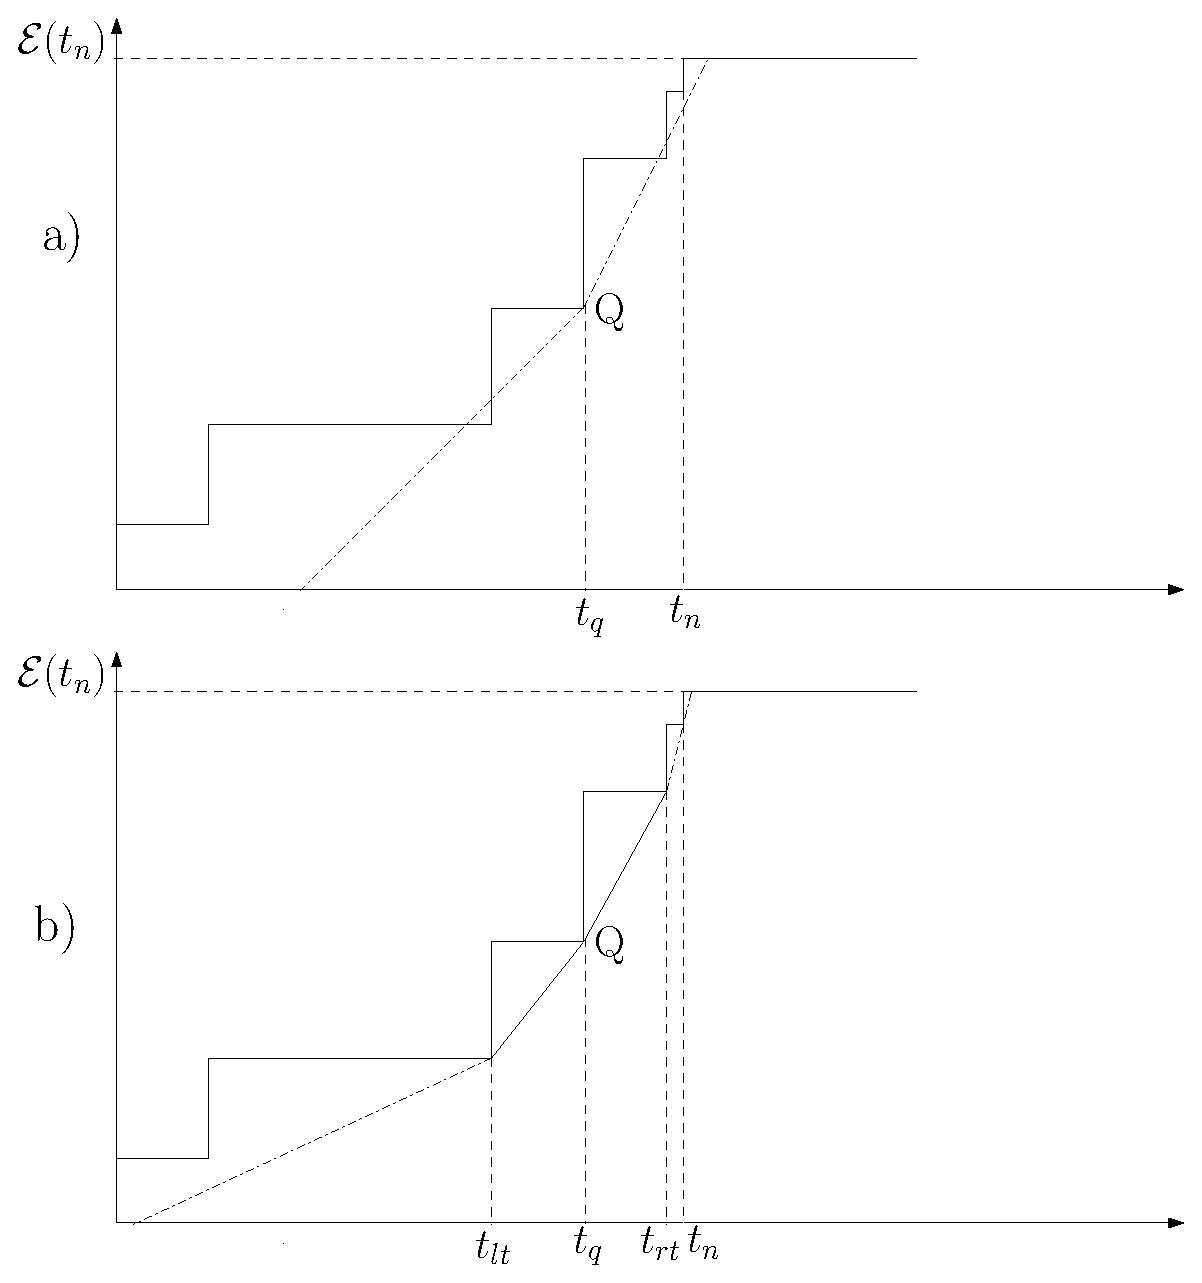
\includegraphics[width=8cm]{theorem1.eps}}
\caption{Figures showing the first two iterations of the algorithm. The dash dotted lines represent the possibly unfeasible powers achieved by solving equation \eqref{xandy}, while the solid lines represent the parts of the policy that go into the final solution.}
\end{figure}


\begin{table}
\begin{minipage}[b]{8cm}
\caption{Offline Algrithm for finding optimal transmission policy, given transmission duration}
\begin{tabular}{p{7cm}}
\hline \textbf{Input}: Bits to transmit $B_0$, transmission duration $T_0$.\\
\hline
\\
\textbf{Initialize:}$B = B_0$, $T = \TRx_0$, DEQUE $S$, hitorig = $0$
\\
% \textbf{While} $Tg(\ETx(n)) < B$
% \\
% \hspace{4mm} $n = n+1$
$n=\displaystyle \argmin_k\left(\left\{t_k | Tg\left(\frac{\ETx(t_k)}{T}\right)\geq B\right\}\right)$
\\
Solve for $\widetilde{T}: \widetilde{T}g\left(\dfrac{\ETx(t_n)}{\widetilde{T}}\right) = B$
\\
$p_0=\dfrac{\ETx(n)}{\widetilde{T}}$
\\
% \textbf{for} $i=0,1,2,...n$ \textbf{do}
% \\
% \hspace{4mm}flag=1
% \\
% \hspace{4mm}\textbf{for} $j=i,i+1,i+2,...,n$ \textbf{do}
% \\
% \hspace{7mm}\textbf{if} $p_0t_j + (\ETx(t_i) - p_0t_i) > \ETx(t_j)$
% \\
% \hspace{10mm}$flag=0$
% \\
% \hspace{10mm}break
% \\
% \hspace{7mm}\textbf{end if}
% \\
% \hspace{4mm}\textbf{end for}
% \\
$q=\displaystyle \argmin_k\left(\left\{ t_k | (\ETx(t_k) - p_0t_k) + p_0t_j \leq \ETx(t_j) \forall j\in[0,n] \right\}\right)$
\\
% \hspace{4mm}\textbf{if} $flag=1$
% \\
% \hspace{7mm}$t_{lt} = t_{rt} = t_i$
% \\
% \hspace{7mm} $S$.append($t_i$)
% \\
% \hspace{7mm}break
% \\
% \hspace{4mm}\textbf{end if}
% \\
% \textbf{end for}
% \\
%$n = \displaystyle \argmax_{k\in\mathbb{N}}\left(\left\{t_k | t_k<\dfrac{E_n - \ETx(t_i) - p_0t_i}{p_0}\right\}\right)$
$t_{lt} = t_{rt} = t_q$
\\
$S$.append($t_q$)
\\
\textbf{while} $B>0$
\\
\hspace{4mm}\textbf{Solve}: $xg\left(\dfrac{\ETx(t_{lt})}{x}\right)+(T-x)g\left(\dfrac{\ETx(t_n)-\ETx(t_{rt})}{T-x}\right) = B_0$
\\
\hspace{4mm}$p_{lt} = \dfrac{\ETx(t_{lt})}{x}$
\\
\hspace{4mm}$p_{rt} = \dfrac{\ETx(t_n)-\ETx(t_{rt})}{T-x}$
\\
\hspace{4mm}$t_{start} = t_{lt} - \dfrac{\ETx(t_{lt})}{p_{lt}}$
\\
\hspace{4mm}$T_{lt} = \{t_i | t_i >t_{start}, t_i < t_{lt}   \}$
\\
\hspace{4mm}$t=0$
\\
\hspace{4mm}\textbf{For} $t_i \in T_{lt}$
\\
\hspace{7mm}\textbf{If} $p_{lt}t_i + (\ETx(t_{lt}) - p_{lt}t_{lt}) > \ETx(t_{i-1})$
\\
\hspace{10mm}$t'_{lt} = t_{lt}$
\\
\hspace{10mm}$t_{lt} = \displaystyle \argmax_{j\in(T_{lt})}\left(\dfrac{\ETx(t_{lt}) - \ETx(j)}{t_{lt}-j}\right)$
\\
\hspace{10mm}$S$.prepend($t_{lt}$)
\\
\hspace{10mm}$t_{start} = t_{lt} - \dfrac{\ETx(t_{lt})}{p_{lt}}$
\\
\hspace{10mm}$t=1$
\\
\hspace{10mm}\textbf{break}
\\
% \hspace{7mm}\textbf{else}
% \\
% \hspace{10mm} $t_{lt} = max(t_{lt} - \dfrac{\ETx(t_lt)}{p_{lt}} , 0)$
% \\
\hspace{7mm}\textbf{end if}
\\
\hspace{4mm}\textbf{End For}
\\
\hspace{4mm}\textbf{if} $t=0$
\\
\hspace{7mm}$t_{lt} = max\left(t_{start} , 0\right)$
\\
\hspace{7mm}\textbf{if} $t_{lt} = 0$ 
\\
\hspace{10mm}hitorig = 1
\\
\hspace{10mm}\textbf{break}
\\
\hspace{4mm}\textbf{end if}
\\
\hspace{4mm}$T_{rt} = \{t_k|t_k>t_{rt}, t_k<t_{rt}+p_{rt}\}$
\\
\hspace{4mm}$u=0$
\\
\hspace{4mm}\textbf{For} $t_i \in T_{rt}$
\\
\hspace{7mm}\textbf{If} $p_{rt}t_i + (\ETx(t_{rt}) - p_{rt}t_{rt}) > \ETx(t_i)$
\\
\hspace{10mm}$t'_{rt} = t_{rt}$
\\
\hspace{10mm}$t_{rt} = \displaystyle \argmin_{j\in(S_{rt})}\left(\dfrac{\ETx(t_j)-\ETx(t_{lrt})}{t_j-t_{rt}}\right)$
\\
\hspace{10mm}$S$.append($t_{rt}$)
\\
\hspace{10mm}$t_{stop} = t_{rt} + \frac{\ETx(E_n)}{p_{rt}}$
\\
\hspace{10mm}$u=1$
\\
\hspace{10mm}\textbf{break}
\\
% \hspace{7mm}\textbf{else}
% \\
% \hspace{10mm} $t_{rt} = t_{rt} + \dfrac{\ETx(t_n)-\ETx(t_rt)}{p_{rt}}$
% \\
% \hspace{10mm}\textbf{If} $t_{rt}>t_{n}$
% \\
% \hspace{13mm}\textbf{While} $t_n < t_{rt}$
% \\
% \hspace{16mm} $n=n+1$
% \\
% \hspace{13mm} \textbf{end while}
% \\
% \hspace{13mm} $t_{rt} = t'_{rt}$
% \\
% \hspace{10mm}\textbf{end for}
% \\
\hspace{7mm}\textbf{end if}
\\
\hspace{4mm}\textbf{End For}
\\
% \textbf{Write the following block in a better way}
% \\
\hspace{4mm}\textbf{if} ($u=0$ and $\ETx(t_{stop}) < \ETx(n) $ )
\\
\hspace{7mm} $n=\displaystyle \argmax_k\left(\left\{t_k | t_k< t_{stop} \right\}\right)$
\\
% \hspace{7mm} $t_{rt} = t_{rt} + \dfrac{\ETx(t_n)-\ETx(t_rt)}{p_{rt}}$
% \\
% \hspace{7mm}\textbf{If} $t_{rt}>t_{n}$
% \\
% \hspace{10mm}\textbf{While} $t_n < t_{rt}$
% \\
% \hspace{13mm} $n=n+1$
% \\
% \hspace{10mm} \textbf{end while}
% \\
% \hspace{7mm} $t_{rt} = t'_{rt}$
% \\
% \hspace{7mm}\textbf{end for}
% \\
\\
\hspace{4mm}\textbf{else if}($u=0$)
\\
\hspace{7mm}$t_{rt} = t_{stop}$
\\
\hspace{7mm}$t_{lt} = t_{start}$
\\
\hspace{4mm}\textbf{end if}
\\
\hspace{4mm} $T = T - (t_{rt}-t'_{lt}) - (t'_{lt} - t_{lt})$
\\
\hspace{4mm}$B = B -  (t'_{lt}-t_{lt})g(\dfrac{\ETx(t'_{lt})-\ETx(t_{lt})}{t'_{lt}-t_{lt}}) - (t_{rt}-t'_{rt})g(\dfrac{\ETx(t_{rt})-\ETx(t'_{rt})}{t_{rt}-t'_{rt}})$
\\
\textbf{end while}
\\
\textbf{if} hitorig = 1
\\
\hspace{4mm}
Apply previous algorithm after $t_{rt}$
\\
\textbf{end if}
\end{tabular}
\end{minipage}
\end{table}
